\documentclass{beamer}
\usepackage{beamerthemeshadow}
\usepackage[ngerman]{babel}
\usepackage[utf8]{inputenc}
\usetheme{Dresden}
\begin{document}
  \title[CodeCover\hspace{105mm}\insertframenumber/\inserttotalframenumber]{CodeCover}
  %\title{CodeCover}
  \author{Michel Meyer und Manuel Schwarz}
  \date{\today}

  \begin{frame}
    \titlepage
  \end{frame}

  \begin{frame}\frametitle{Inhalt}\tableofcontents
  \end{frame}


  \section{Einleitung}
  \subsection{Motivation}
  \begin{frame}\frametitle{Motivation}
    \begin{itemize}
      \item 
      \item 
      \item 
      \item 
    \end{itemize}
  \end{frame}

  \subsection{Überblick}
  \begin{frame}\frametitle{Überblick}
    \begin{itemize}
      \item 
      \item 
      \item 
      \item 
    \end{itemize}
  \end{frame}

  \section{CodeCover allgemein}
  \subsection{Einsatzzweck}
  \begin{frame}\frametitle{White- bzw. Glass-Box Testing}
    \begin{itemize}
      \item 
      \item 
      \item 
      \item 
      \item 
      \item 
    \end{itemize}
  \end{frame}

  \subsection{Allgemeine Informationen}
  \begin{frame}\frametitle{Download und Toolinfos}
    \begin{itemize}
      \item Quelle: kostenlos unter \texttt{codecover.org}
      \item letzte Version (Stand: März 2011): \texttt{CodeCover 1.0.1.2} (knapp 3 MB)
      \item Lizenz: Eclipse Public Licence (EPL)
      \item Plattformen: Kommandozeile (Linux, Windows, Mac OS) sowie Eclipse- und Ant-Integration
      \item Programmiersprachen: \texttt{Java} und \texttt{COBOL}
    \end{itemize}
  \end{frame}

  \subsection{Installation (Eclipse)}
  \begin{frame}
    \frametitle{Installation}
    \begin{columns}
      \begin{column}{4cm}
        \begin{itemize}
          \item \texttt{Eclipse} starten
          \item \texttt{Help} $\rightarrow$ \texttt{Install New Software\dots}
          \item URL: \texttt{http://update.codecover.org/} eingeben
          \item \texttt{CodeCover} auswählen
        \end{itemize}
        \vspace{2cm}
      \end{column}
      \begin{column}{6cm}
        \begin{overprint}
          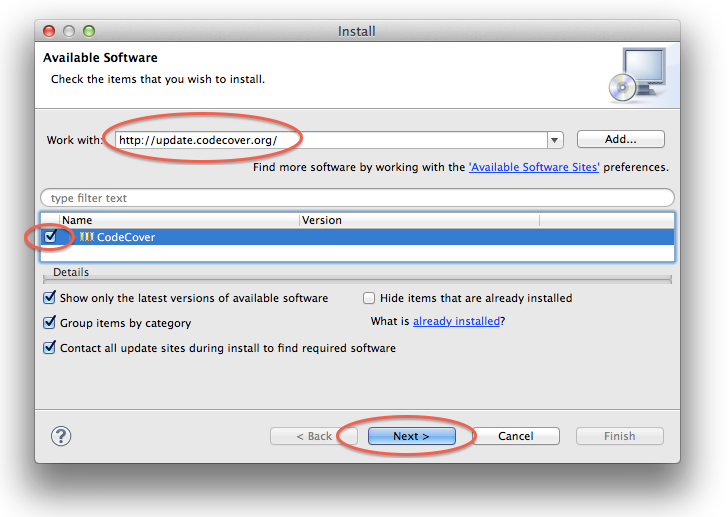
\includegraphics[width=7cm]{pictures/install.png}
        \end{overprint}
      \end{column}
    \end{columns}
  \end{frame}

  \begin{frame}
    \frametitle{CodeCover aktivieren}
    \begin{columns}
      \begin{column}{4cm}
        \begin{itemize}
          \item Rechtsklick auf gewünschtes Projekt
          \item \texttt{CodeCover} auswählen und aktivieren
          \item die gewünschten Kriterien auswählen
        \end{itemize}
        \vspace{2cm}
      \end{column}
      \begin{column}{6cm}
        \begin{overprint}
          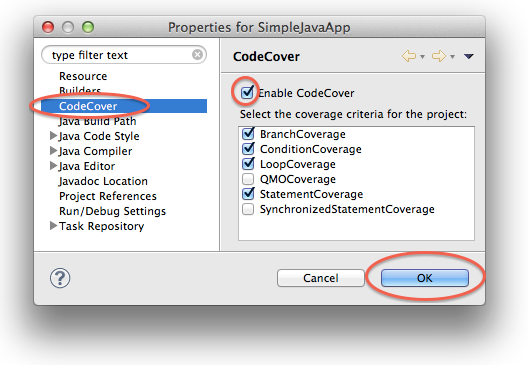
\includegraphics[width=6cm]{pictures/activate.png}
        \end{overprint}
      \end{column}
    \end{columns}
  \end{frame}

  \begin{frame}
    \frametitle{Zu prüfende Klassen auswählen}
    \begin{columns}
      \begin{column}{5cm}
        \begin{itemize}
          \item zu testende Klassen auswählen
          \item Rechtsklick $\rightarrow$ \texttt{Use For Coverage Measurement}
        \end{itemize}
        \vspace{2cm}
      \end{column}
      \begin{column}{5cm}
        \begin{overprint}
          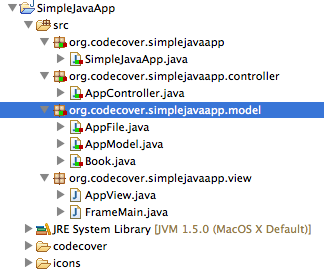
\includegraphics[width=4cm]{pictures/testclasses.png}
        \end{overprint}
      \end{column}
    \end{columns}
  \end{frame}

  \begin{frame}
    \frametitle{Ausführen}
    \begin{columns}
      \begin{column}{4cm}
        \begin{itemize}
          \item \texttt{Run} $\rightarrow$ \texttt{Run Configurations\dots}
          \item \texttt{Run with CodeCover} auswählen
          \item Ausführen
        \end{itemize}
        \vspace{2cm}
      \end{column}
      \begin{column}{6cm}
        \begin{overprint}
          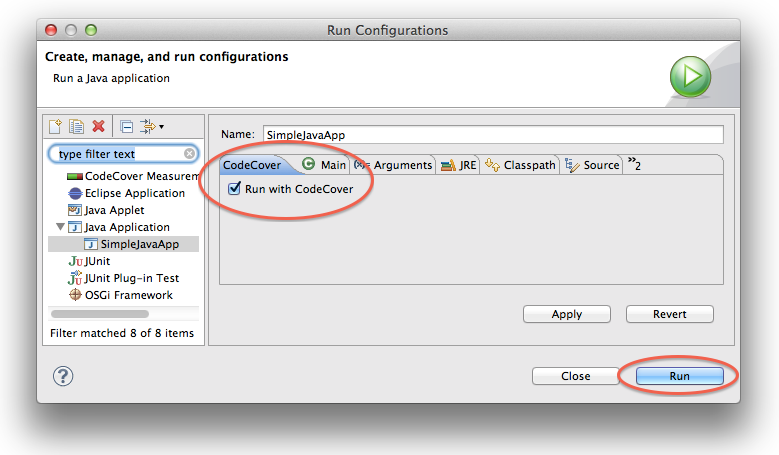
\includegraphics[width=7cm]{pictures/runconfigurations.png}
        \end{overprint}
      \end{column}
    \end{columns}
  \end{frame}

  \section{Funktionsweise}
  \subsection{Tests}
  \begin{frame}\frametitle{Testarten}
  CodeCover deckt folgende Tests ab:
    \begin{itemize}
      \item Bedingungsüberdeckung
      \item Zweigüberdeckung
      \item Schleifenüberdeckung
      \item Anweisungsüberdeckung
      \item Ternärer Operator Überdeckung
      \item Synchronisationsüberdeckung
    \end{itemize}
  \end{frame}

  \subsection{Technische Integration}
  \begin{frame}\frametitle{Benutzung}
    \begin{itemize}
      \item Kommandozeile (Report erstellen)
      \item Eclipse (verschiedene Views + Report)
      \item Ant
      \item JUnit
    \end{itemize}
  \end{frame}

  \begin{frame}\frametitle{Farbkodierung}
    \begin{columns}
      \begin{column}{5cm}
        \begin{itemize}
          \item grün: komplette Abdeckung
          \item gelb: Teilabdeckung
          \item rot: wird nicht evaluiert
        \end{itemize}
        \vspace{1cm}
      \end{column}
      \begin{column}{5cm}
        \begin{overprint}
          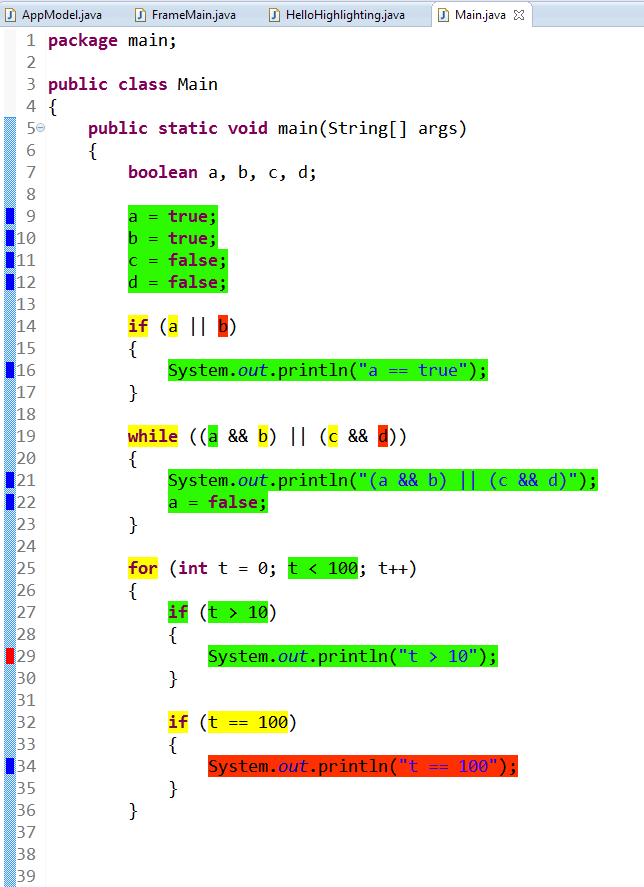
\includegraphics[height=65mm]{pictures/farben.png}
        \end{overprint}
      \end{column}
    \end{columns}
  \end{frame}

  \section{CodeCover Demo}
  \subsection{Kommandozeile}
  \begin{frame}\frametitle{einfaches Beispiel}
    \centering \Huge{DEMO}\\
  \end{frame}

  \subsection{Eclipse}
  \begin{frame}\frametitle{komplexes Beispiel}
    \centering
    \Huge{DEMO}\\
    \centering
    \normalsize{\texttt{SimpleJavaApp}}\\
  \end{frame}


  \section{Fazit}
  \begin{frame}\frametitle{Zusammenfassung und Fazit}
    \begin{itemize}
      \item gute Eclipse-Integration
      \item einfaches Generieren und Zusammenfassen von Testfällen
      \item verschiedene nützliche Views in Eclipse
      \item keine Weiterentwicklung seit fast 2 Jahren
      \item nur \texttt{Java} und \texttt{COBOL} werden unterstützt
      \item evtl. Alternativen suchen
    \end{itemize}
  \end{frame}



\end{document}

 % \begin{block}{title of the bloc}
 % bloc text
 % \end{block}

 % \begin{exampleblock}{title of the bloc}
 % bloc text
 % \end{exampleblock}


 % \begin{alertblock}{title of the bloc}
 % bloc text
 % \end{alertblock}
